\chapter{Timing Analysis and Anomalies}

A \textit{counterintuitive timing anomaly}, referred to as a \textit{timing anomaly (TA)} in this work, is a phenomenon where a locally favorable condition results in a globally worse outcome (for example, a cache hit leading to a program slowdown). In contrast to counterintuitive anomalies, there also exist amplification timing anomalies, where the timing delay is greater than expected; however, this work focuses solely on counterintuitive anomalies. The concept of timing anomalies was first introduced by Lundqvist and Stenstr\"om in 1999 \cite{lundqvist_timing_1999} in the context of timing analysis. TAs are architectural features that complicate the accurate analysis of timing behavior. Such anomalies can significantly impact execution time in ways not captured by worst-case execution time (WCET) analysis. Particularly problematic is the so-called domino effect, also described by Lundqvist and Stenstr\"om, which can lead to an unbounded slowdown due to the propagation of timing anomalies.

\section{Evolution of TA-definitions}



Despite the fact that timing anomalies have been known for a long time, the exact TA definition is a subject to debates. Since 1999 several attempts were made to formalize the notion of TA, some of them being more focused on the exact microarchitecture (like \cite{gruin_minotaur_2023}) and some being more abstract and general (like \cite{binder_definitions_2022}, \cite{hahn_design_2020}). In this section we are giving an overview of existing definitions comparing their strengths and weaknesses.

\subsection{Step Heights}
Gebhard \cite{gebhard_timing_2012} defines timing anomalies based on the comparison of local and global execution times. Specifically, a timing anomaly is present if an earlier instruction exhibits a shorter local execution time, while a later instruction in the same trace has a longer global execution time compared to another trace.

Figure \ref{fig:step-good} illustrates this definition using Example \ref{ex:simple-ta}. The orange on the top arrow indicates the local execution time of instruction $A$. The global execution times for instruction $D$ differ between traces $\alpha$ and $\beta$ (13 and 11, respectively).

\begin{figure}[!htb]
    \centering
    \begin{subfigure}[t]{0.5\textwidth}
        \centering
        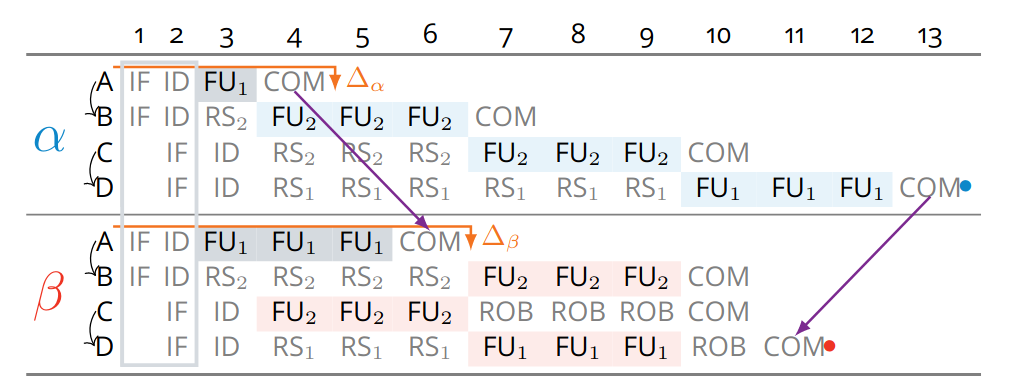
\includegraphics[width=\textwidth]{figures/step-func-good.png}
        \caption{Interpretation of Example \ref{ex:simple-ta} using Gebhard's definition}
        \label{fig:step-good}
    \end{subfigure}
    \hfill
    \begin{subfigure}[t]{0.49\textwidth}
        \centering
        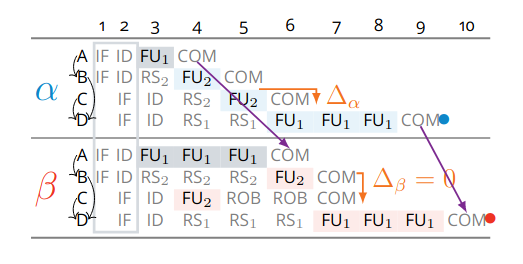
\includegraphics[width=\textwidth]{figures/step-func-bad.png}
        \caption{Counterexample to the definition}
        \label{fig:step-bad}
    \end{subfigure}
    \caption{Gebhard's definition applied to execution traces (from \cite{binder_definitions_2022})}
    \label{fig:step}
\end{figure}

In his thesis \cite{binder_definitions_2022}, Binder provides a counterexample (Figure \ref{fig:step-bad}), where it is clear that there is no TA (trace $\beta$ has both unfavorable variation and longer execution time). However, Gebhard's definition signals an anomaly because of shorter local execution time of instruction $C$ in trace $\beta$.

This poses a question whether it is reasonable to capture a local execution time as difference between instruction completion times. 

\subsection{Step-functions Intersections}

\begin{figure}[H]
    \centering
    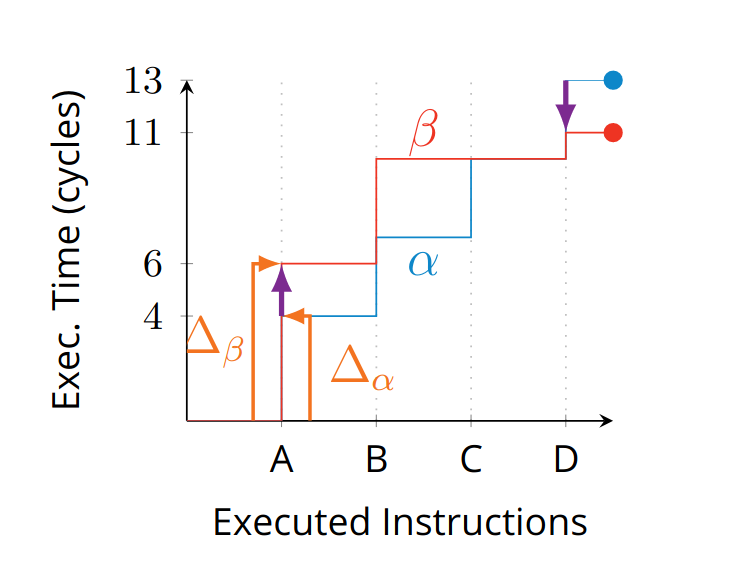
\includegraphics[width=0.4\textwidth]{figures/step-functions.png}
    \caption{Execution time as step functions (from \cite{binder_definitions_2022})}
    \label{fig:exec-time-step-fun}
\end{figure}

A similar definition is proposed by Cassez et al. \cite{cassez_what_2012}. The difference is that only the global execution time is taken into account. Thus, a TA arises when the step-functions (that map instructions to their absolute completion time) of two traces intersect. For example, Figure \ref{fig:exec-time-step-fun} shows the execution times as step functions from Example \ref{ex:simple-ta}. The two functions intersect between $C$ and $D$, thus signalling an anomaly.


\begin{figure}[!htb]
    \centering
    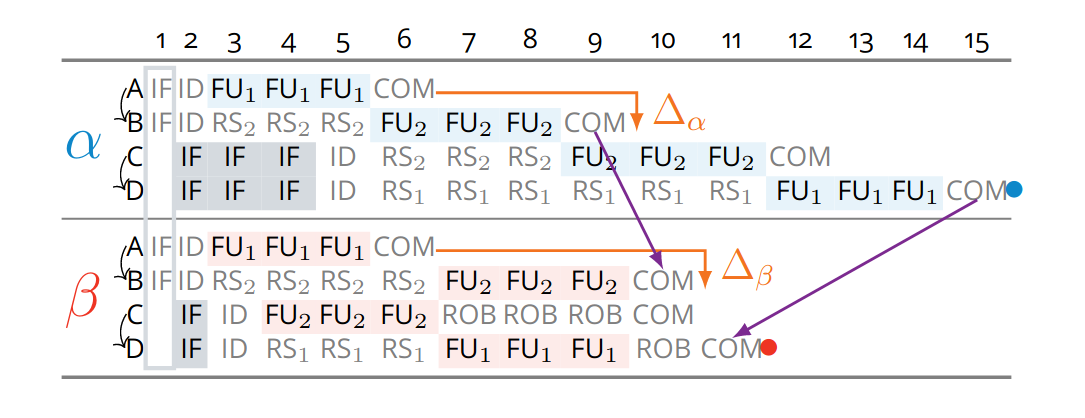
\includegraphics[width=\textwidth]{figures/step-func-2-bad.png}
    \caption{Contradicting result of Cassez's definition (from \cite{binder_definitions_2022})}
    \label{fig:step-2}
\end{figure}

This definition also leads to a misleading effect with a scenario found by Binder \cite{binder_definitions_2022}. Figure \ref{fig:step-2} illustrates this by comparing two traces. The step-functions of traces $\alpha$ and $\beta$ intersect, however there is no counterintuitive TA happening as $\alpha$ is both longer and has a longer latency for the IF stage of instructions $C$ and $D$.

\subsection{Component Occupation}

An alternative approach is proposed by Kirner et al. \cite{kirner_precise_2009}. In their work the idea is to partition hardware into components and for each one define the occupation by instruction (for how many cycles it processes the instruction). A TA arises when a shorter component occupation coincides with a longer execution time in a chosen trace. For example, take Figure \ref{fig:step-good} and consider $FU_1$ and $FU_2$ as hardware components. In total, $FU_1$ is occupied for 4 cycles in trace $\alpha$ and 6 cycles in trace $\beta$. In the same time the execution time of $\alpha$ is longer, so a TA is identified.

A main challenge with this definition is choosing the right components. The authors do not give a formal way to define what a component is or what properties it should have. For example, in the previous case, it is not clear if the chosen partitioning is valid, since functional units like $FU_1$ and $FU_2$ are controlled by the processor's instruction scheduling and thus are not fully independent. Another problem is that the occupation time of a component can change because of instructions that are not directly related to the timing anomaly. For instance, an earlier or later instruction, which does not affect the total execution time, might still reduce the occupation time of a component and cause a false positive. Similarly, false negatives can also occur. Additionally, if a resource switch happens (for example, an instruction is executed on a different functional unit in another trace), it can make the comparison of occupation times unreliable and further complicate the detection of timing anomalies.

\TODO{counterexample}

% \subsection{Instruction Locality}


\TODO{Instruction Locality}

% \subsection{Progress-based definition}

\TODO{Progress-based definition}

% Hahn and Reineke \cite{hahn_design_2020} introduce the notion of progress, ... \cite{gruin_minotaur_2023}

\subsection{Event Time Dependency Graph}

Binder et al. \cite{binder_definitions_2022} define TAs using the notion of causality between events in an execution trace. In this work, a superscalar OoO pipeline is considered. The processor state is described as a composition of the states of each of the resources: \textit{IF, ID, set of RS, set of FU, ROB, COM}. Each component holds information about the instruction it is currently processing, including required registers and remaining clock cycles.

The notion of an event is introduced based on qualitative changes in the pipeline associated with an instruction progressing through stages. An event from an execution trace (denoted as $e \in Events(\alpha)$) is a triple $(i,r,t)$, where $i$ is the instruction to which the event is related, $r$ is the associated resource and the action (acquisition or release), and $t$ is a timestamp corresponding to the clock cycle when the event occurs.

In the proposed framework, events correspond to the \textit{IF, ID, FU}, and \textit{COM} pipeline stages. For each instruction, there are seven types of events: $\IFa$, $\IFr$, $\IDa$, $\IDr$, $\FUa$, $\FUr$, and $COM$. The symbol $\uparrow$ denotes the acquisition of a resource, while $\downarrow$ indicates its release. $COM$ represents the acquisition of the commit stage; its release always occurs one clock cycle later, and since no subsequent stages exist, it is not further considered in the framework.

\textbf{Latency} is defined as the time difference between the acquisition and release of a resource. Each instruction passes through the same pipeline stages and is associated with the corresponding events. Thus, for each pair of traces corresponding to the same program, the sets of events differ only in their timestamps or, potentially, in the functional unit (FU) used, although resource switching is not modeled within this framework. Consequently, for each event in one trace, there exists a corresponding event in the other. Formally, this correspondence is defined by the function $CospEvent: Events(\alpha) \rightarrow Events(\beta)$.

\textbf{Variation} refers to the observation that the latency in one trace differs from the latency of the corresponding events in the other trace. For a pair of traces $\alpha$ and $\beta$, the variation is considered favorable for $\alpha$ if the latency in $\alpha$ is smaller than in $\beta$.

Variations are considered as the source of timing anomalies. They may represent different memory behaviors (e.g., cache hit or miss) for fetch and memory accesses in FU. Other sources of timing anomalies, such as memory bus contention or branching, are not considered in this framework.

The \textbf{Event Time Dependency Graph (ETDG)} of a trace $\tau$, denoted as $G(\tau) = (\mathcal{N}, \mathcal{A})$, consists of a set of nodes $\mathcal{N} = Events(\tau)$ and a set of arcs $\mathcal{A} \subseteq \mathcal{N} \times \mathcal{N} \times \mathbb{N}$.

An arc is a triple $(e_1, e_2, w)$ written as $e_1 \xrightarrow{w} e_2$, where $e_1$ is the source event node, $e_2$ is the destination node, and $w$ is a lower bound of the delay between the two events. The arc means that at least $w$ clock cycles must pass between $e_1$ and $e_2$. 

Arcs are derived from a set of rules:
\begin{enumerate}
    \item \textbf{Order of pipeline stages}
    
    Every instruction goes through the pipeline stages in a fixed order: first it is fetched, then decoded, then executed and only then committed. This creates following dependencies for a given instruction $I$:

    \begin{itemize}
        \item $(I, \IFr, t_1) \xrightarrow{0} (I, \IDa, t_2)$
        \item $(I, \IDr, t_3) \xrightarrow{0} (I, \FUa, t_4)$
        \item $(I, \FUr, t_5)  \xrightarrow{0} (I, COM, t_6)$
    \end{itemize}

    \item \textbf{Resource use}

    An instruction takes one or several clock cycles to go through each stage and cannot pass them faster.

    \begin{itemize}
        \item $(I, \IFa, t_0) \xrightarrow{lat_{IF}} (I, \IFr, t_1)$
        \item $(I, \IDa, t_2) \xrightarrow{1} (I, \IDr, t_3)$
        \item $(I, \FUa, t_4)  \xrightarrow{lat_{FU}} (I, \FUr, t_5)$
    \end{itemize}

    $lat_{IF}$ and $lat_{FU}$ are the latencies of IF and FU stages respectively that come from how many clock cycles are required to fetch or execute a given instruction based on was it cache hit or miss for memory instructions.

    $lat_{IF} = t_1 - t_0$, $lat_{FU} = t_5 - t_4$

    \item \textbf{Instruction order}
    
    The in-order part of the pipeline is constrained by instruction order. Thus, for successive instructions $I_1$ and $I_2$:

    $(I_1,  \uparrow RES, t) \xrightarrow{0} (I_2, \uparrow RES, t'), RES \in \{IF, ID, COM\}$


    \item \textbf{Data dependencies}
    
    A RAW dependency between $I_1$ and $I_2$ restricts the execution order of the instructions:  $(I_1, \FUr, t) \xrightarrow{0} (I_2, \FUa, t')$.
    
    \item \textbf{Resource contention}
    
    Also some instruction can be delayed because of limited resources. For instance, FU contention happens when $I_1$ and $I_2$ use the same FU, and it is busy by $I_1$ at the moment when $I_2$ is ready. This creates $(I_1, \FUr, t) \xrightarrow{0} (I_2, \FUa, t')$. 

    Resource contention can also be caused by reaching the capacity limit of ROB or RS. 
\end{enumerate}
The \textbf{causality graph} is derived from the ETDG by removing unnecessary edges. For each event, we keep only the most relevant constraint. Only arcs of the form $e_1 \xrightarrow{e_2.time - e_1.time} e_2$ are left. Also, arcs related to variations are excluded, as in the case of a variation the delay of acquisition is induced by the hidden hardware state and not by the scheduling.

A \textbf{timing anomaly}, according to Binder, consists of three observations: variation, causality, and slowdown. If a trace exhibits a favorable variation and in its causal region there is an event that is delayed, then a TA is signaled.

Formally, a TA is observed on a pair of traces $\alpha$ and $\beta$ if there exists a favorable variation in $\alpha$ relative to $\beta$. Let $\downarrow e_\alpha$ and $\downarrow e_\beta$ be the events corresponding to the end of the variation in both traces. If there exist events $e'_\alpha$ and $e'_\beta$, where $e'_\beta = CospEvent(e'_\alpha)$ and there is a path in the causality graph of $\alpha$ between $\downarrow e_\alpha$ and $e'_\alpha$, such that $\Delta(\downarrow e_\beta,e'_\beta) < \Delta(\downarrow e_\alpha,e'_\alpha)$, where $\Delta$ is the delay between the two events, then a TA is signaled.

\begin{figure}[htbp]
    \centering
    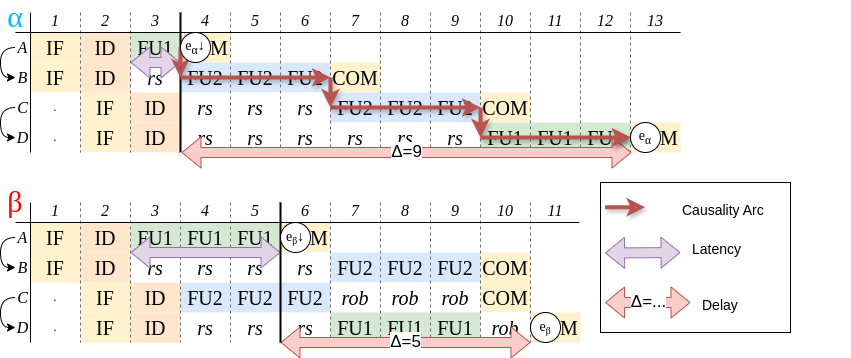
\includegraphics[width=0.8\textwidth]{figures/multiscalar_ta_causality.png}
    \caption{Causality-based TA detection applied to Example \ref{ex:simple-ta}. $e_\alpha\downarrow = (A, \FUr, 4), e_\beta\downarrow = (A, \FUr, 6), e_\alpha = (A, COM, 13), e_\beta = (A, COM, 11)$. Purple arrow denotes latency which has a variation between two traces. Light red arrow shows delay between events which is greater in favorable trace. Causality in path $\alpha$ is marked by dark red arrows.}
    \label{fig:multiscalar-ta-causality}
\end{figure}

\begin{figure}[htbp]
    \centering
    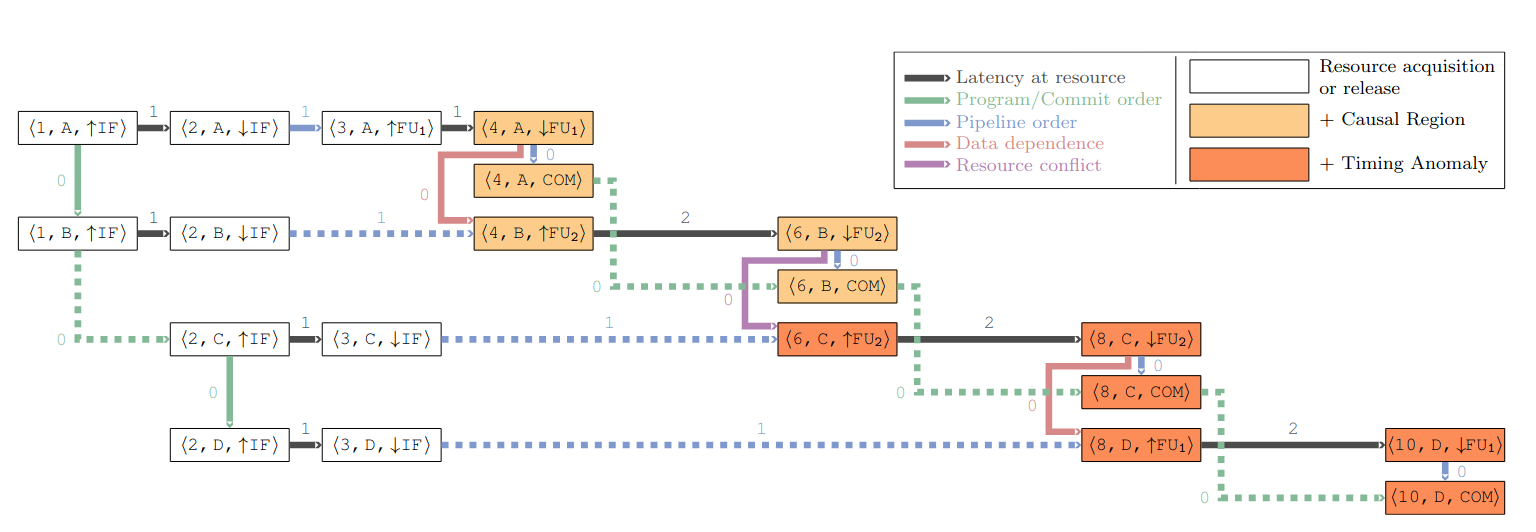
\includegraphics[width=\textwidth]{figures/ETDG.png}
    \caption{Complete ETDG for trace $\alpha$ from Figure \ref{fig:multiscalar-ta-causality}, trace $\alpha$ (from \cite{CAOTIC-report}).}
    \label{fig:ETDG}
\end{figure}

Figure \ref{fig:multiscalar-ta-causality} shows how the framework captures a TA for Example \ref{ex:simple-ta}. Figure \ref{fig:ETDG} presents the complete ETDG for trace $\alpha$, with different dependency rules highlighted in different colors. The arcs reflecting causality are depicted with solid lines.

In contrast to other definitions, this one measures relative time from the acquisition of the resource instead of global time. This approach allows the separation of different variations and isolates the part of the trace that experiences the TA effect.


% \section{TA-classifications}
\section{Conclusion}

In this chapter, we reviewed the evolution of timing anomaly definitions, highlighting their strengths and limitations. We discussed approaches based on step heights, step-function intersections, component occupation, and causality graphs. While early definitions often led to misleading or ambiguous results, more recent formalizations -- such as the event time dependency graph -- offer a more precise and nuanced understanding of timing anomalies. Notably, Binder's event-based definition is the most promising in the context of branch prediction, as its flexible set of rules can be adapted to architectural details, enabling accurate modeling of complex behaviors. This progression underscores the complexity of accurately capturing timing anomalies and the importance of rigorous, architecture-aware definitions for reliable timing analysis.